% --------------------------------------------------------------------------
% Formatvorlage f�r Diplomarbeiten der FHWT
% --------------------------------------------------------------------------
% 	Angelehnt an die Word-Vorlage von Herrn St�hrenberg
% 	Download unter http://www.atlando.de/fhwt.htm
%
% 	erstellt von Stefan Macke. 22.10.2007
% 	http://blog.stefan-macke.de


% Meta-Informationen -------------------------------------------------------
%		Informationen �ber das Dokument, wie z.B. Titel, Autor, Matrikelnr. etc
%		werden in der Datei _Meta.tex definiert und k�nnen danach global
%		verwendet werden.
% --------------------------------------------------------------------------
% Informationen ------------------------------------------------------------
% 	Definition von globalen Parametern, die im gesamten Dokument verwendet
% 	werden k�nnen (z.B auf dem Deckblatt etc.).
% --------------------------------------------------------------------------
\newcommand{\titel}{Entwickeln von Anwendungen f�r Hand Held}
\newcommand{\untertitel}{...}
\newcommand{\art}{Seminar Arbeit}
\newcommand{\fachgebiet}{Wirtschaftsinformatik}
\newcommand{\autor}{Andreas Gr�nenfelder}
\newcommand{\autorTwo}{Micha Sch�nenberger}
\newcommand{\studienbereich}{Wirtschaftsinformatik}
\newcommand{\matrikelnr}{12 34 56}
\newcommand{\erstgutachter}{Christian Vils}
%\newcommand{\zweitgutachter}{Dipl.-Inf. Lukas Podolski}
\newcommand{\jahr}{2012}

% Eigene Befehle und typographische Auszeichnungen f�r diese
\newcommand{\todo}[1]{\textbf{\textsc{\textcolor{red}{(TODO: #1)}}}}

\newcommand{\AutorZ}[1]{\textsc{#1}}
\newcommand{\Autor}[1]{\AutorZ{\citeauthor{#1}}}

\newcommand{\NeuerBegriff}[1]{\textbf{#1}}

\newcommand{\Fachbegriff}[1]{\textit{#1}}
\newcommand{\Prozess}[1]{\textit{#1}}
\newcommand{\Webservice}[1]{\textit{#1}}

\newcommand{\Eingabe}[1]{\texttt{#1}}
\newcommand{\Code}[1]{\texttt{#1}}
\newcommand{\Datei}[1]{\texttt{#1}}

\newcommand{\Datentyp}[1]{\textsf{#1}}
\newcommand{\XMLElement}[1]{\textsf{#1}}


% Abk�rzungen mit korrektem Leerraum
\newcommand{\vgl}{Vgl.\ }
\newcommand{\ua}{\mbox{u.\,a.\ }}
\newcommand{\zB}{\mbox{z.\,B.\ }}
\newcommand{\bs}{$\backslash$}








% Dokumentenkopf -----------------------------------------------------------
% 	Diese Vorlage basiert auf "scrreprt" aus dem koma-script.
%		Die Option draft sollte beim fertigen Dokument ausgeschaltet werden.
% --------------------------------------------------------------------------
\documentclass[
	11pt,								% Schriftgr��e
	DIV10,
	german,							% f�r Umlaute, Silbentrennung etc.
	a4paper,         		% Papierformat
	oneside,						% einseitiges Dokument
	titlepage,					% es wird eine Titelseite verwendet
	halfparskip,				% Abstand zwischen Abs�tzen (halbe Zeile)
	normalheadings,			% Gr��e der �berschriften verkleinern
	liststotoc,					% Verzeichnisse im Inhaltsverzeichnis auff�hren
	bibtotoc,						% Literaturverzeichnis im Inhaltsverzeichnis auff�hren
	idxtotoc,						% Index im Inhaltsverzeichnis auff�hren
	tablecaptionabove,	% Beschriftung von Tabellen unterhalb ausgeben
	final								% Status des Dokuments (final/draft)
]{scrreprt}


% Ben�tigte Packages -------------------------------------------------------
%		Weitere Packages, die ben�tigt werden, sind in die Datei Packages.tex
%		"ausgelagert", um die Vorlage m�glichst �bersichtlich zu halten.
% --------------------------------------------------------------------------
%--------------------------------------------------------------------- INFORMATIONEN -----------------------------------------------------------------------------------------------------------------------
%																															|
% 	Definition von globalen Parametern, die im gesamten Dokument verwendet																|
% 	werden k�nnen (z.B auf dem Deckblatt etc.).																						|
% ----------------------------------------------------------------------------------------------------------------------------------------------------------------------------------------------------------------------



\usepackage{cite}								%f�r Literaturverzeichnis
\usepackage{tocbasic}




%------------------------------------------------------- FORMATIERUNG KOPF- UND FUSSZEILE ----------------------------------------------------------------------------------------------------
%																															|
\usepackage									%																				|
[automark,									%Automatische Kopfzeile      															|
%headtopline,									%Linie �ber dem Seitenkopf      														|
%plainheadtopline,								%Plain, Linie �ber dem Seitenkopf      													|
headsepline,									%Linie zwischen Kopf und Textk�rper      													|
ilines,										% Trennlinie linksb�ndig ausrichten      													|
%plainheadsepline,								%Plain, Linie zwischen Kopf und Textk�rper      											|
footsepline,									%Linie zwischen Textk�rper und Fuss      													|
plainfootsepline,   								%Plain, Linie zwischen Textk�rper und Fuss      											|
%footbotline,									%Linie unter dem Fuss      															|
%plainfootbotline   								%Plain, Linie unter dem Fuss      														|
]{scrpage2}									%																				|
% 																															|
% ----------------------------------------------------------------------------------------------------------------------------------------------------------------------------------------------------------------------


%---------------------------------------------------------------- ANPASSUNG LANDESSPRACHE-------------------------------------------------------------------------------------------------------
%																															|
% Verwendet globale Option german siehe \documentclass																				|
\usepackage{babel}  							%						      														|
% 																															|
% ----------------------------------------------------------------------------------------------------------------------------------------------------------------------------------------------------------------------


%---------------------------------------------------------------------------------- UMLAUTE----------------------------------------------------------------------------------------------------------------------
%																															|
\usepackage[latin1]{inputenc}						%Unterst�tzung erweiterter Zeichens�tze mit  unterschiedlichen Kodierungen (z. B. �, �, � usw.)		|
\usepackage[T1]{fontenc}							%Dadurch ist auch sichergestellt, dass in einem PDF Umlaute gefunden werden.					|
%\usepackage{ae} 								% "sch�neres" �																	|
\usepackage{textcomp} 							% Euro-Zeichen etc.																	|
%																															|
% @inputenc:																													|
% inputenc (Einbindung mit \usepackage[latin1]{inputenc}) ist f�r die Unterst�tzung erweiterter Eingabe-Zeichens�tze mit ihren unterschiedlichen Kodierungen	|
%(z. B. �, �, � usw.). Es dient der Umwandlung einer beliebigen Eingabe-Zeichenkodierung in eine interne LaTeX-Standardsprache. Neben latin1 gibt es noch	|
%weitere Codierungen, so zum Beispiel applemac (eine Kodierung, die h�ufig f�r Textdateien unter Mac OS verwendet wurde) oder utf8 f�r UTF-8-kodierte	|
%Dateien. Im Austausch kann es aufgrund der unterschiedlichen Eingabe-Zeichenkodierung zu Problemen kommen.									|
% 																															|
% ----------------------------------------------------------------------------------------------------------------------------------------------------------------------------------------------------------------------


%---------------------------------------------------------------------------------- GRAFIKEN---------------------------------------------------------------------------------------------------------------------
%																															|
\usepackage[dvips,final]{graphicx}						%Einbinden von EPS-Grafiken [draft oder final]										|
\graphicspath{{pictures/}} 								% Hier liegen die Bilder des Dokuments												|
%																															|
% ----------------------------------------------------------------------------------------------------------------------------------------------------------------------------------------------------------------------



\usepackage{amsmath,amsfonts}						% Befehle aus AMSTeX f�r mathematische Symbole z.B. \boldsymbol \mathbb ----

\usepackage{multirow}								%Packages f�r Tabellen



% Weitere Zeichen z.B. \textcelsius \textordmasculine \textsurd \textonehalf 
% \texteuro \texttimes \textdiv ... aus textcomp.sty
% siehe >>Schnell ans Ziel mit \LaTeXe<< von J�rg Knappen
% (Oldenbourg, M�nchen und Wien 1997, ISBN 3-486-24199-0)
% \usepackage{tccompat}
	
%---------------------------------------------------------------------------- OWN COLORS---------------------------------------------------------------------------------------------------------------------
%																															|
\usepackage{colortbl}   								% F�r eigene Color Definitionen (Definitionen siehe Meta)								|
\definecolor{darkgrey}{rgb}{0.8,0.8,0.8}					% 																			|
%																															|
% ----------------------------------------------------------------------------------------------------------------------------------------------------------------------------------------------------------------------


\usepackage{makeidx}								% F�r Index-Ausgabe; \printindex


%---------------------------------------------------------------------------- ZEILENABST�NDE UND SEITENR�NDER--------------------------------------------------------------------------------
%																															|

% Einfache Definition der Zeilenabst�nde und Seitenr�nder etc. -------------
\usepackage{setspace}								% hat zur Ben�tzung 3 Optionen: [singlespacing, onehalfspacing, doublespacing]				|
\usepackage{geometry}	


% Symbolverzeichnis --------------------------------------------------------
% 	Symbolverzeichnisse bequem erstellen, beruht auf MakeIndex.
% 		makeindex.exe %Name%.nlo -s nomencl.ist -o %Name%.nls
% 	erzeugt dann das Verzeichnis. Dieser Befehl kann z.B. im TeXnicCenter
%		als Postprozessor eingetragen werden, damit er nicht st�ndig manuell
%		ausgef�hrt werden muss.
%		Die Definitionen sind ausgegliedert in die Datei Abkuerzungen.tex.
% --------------------------------------------------------------------------
\usepackage[intoc]{nomencl}
  \let\abbrev\nomenclature
  \renewcommand{\nomname}{Abk�rzungsverzeichnis}
  \setlength{\nomlabelwidth}{.25\hsize}
  \renewcommand{\nomlabel}[1]{#1 \dotfill}
  \setlength{\nomitemsep}{-\parsep}


\usepackage{floatflt}								% Zum Umflie�en von Bildern


% Zum Einbinden von Programmcode --------------------------------------------
\usepackage{listings}
\usepackage{xcolor} 
\definecolor{hellgelb}{rgb}{1,1,0.9}
\definecolor{colKeys}{rgb}{0,0,1}
\definecolor{colIdentifier}{rgb}{0,0,0}
\definecolor{colComments}{rgb}{1,0,0}
\definecolor{colString}{rgb}{0,0.5,0}
\lstset{%
    float=hbp,%
    basicstyle=\texttt\small, %
    identifierstyle=\color{colIdentifier}, %
    keywordstyle=\color{colKeys}, %
    stringstyle=\color{colString}, %
    commentstyle=\color{colComments}, %
    columns=flexible, %
    tabsize=2, %
    frame=single, %
    extendedchars=true, %
    showspaces=false, %
    showstringspaces=false, %
    numbers=left, %
    numberstyle=\tiny, %
    breaklines=true, %
    backgroundcolor=\color{hellgelb}, %
    breakautoindent=true, %
%    captionpos=b%
}

% Lange URLs umbrechen etc. -------------------------------------------------
\usepackage{url}




% Wichtig f�r korrekte Zitierweise ------------------------------------------
%%\usepackage[square]{natbib}
% Quellenangaben in eckige Klammern fassen ---------------------------------
%%\bibpunct{[}{]}{;}{a}{}{,~}


%\usepackage{jurabib}
%\jurabibsetup{authorformat=smallcaps,% Autor in Kapit�lchen              
%              %authorformat=year,
%              authorformat=citationreversed,% Im Zitat Vorname vorne
%              authorformat=indexed,% Autor in Index
%              authorformat=and,% Autoren mit "," und "und" abgetrennt
%              authorformat=firstnotreversed,%
%              authorformat=reducedifibidem,% Bei Verweis nur Nachname. 
%              %superscriptedition=all,% Auflage hochgestellt
%              %citefull=first,% Erstzitat voll
%              titleformat=italic,              
%              titleformat=all,
%              titleformat=colonsep,% Doppelpunkt zwischen Aut. u. Titel
%              ibidem=strict,% Ebenda pro Doppelseite
%              see,% Das zweite Argument ist optional f�r "Vgl." etc.
%              commabeforerest,% Komma vor Seitenzahl
%              %howcited=compare,%
%              %bibformat=ibidem,% Strich bei widerholtem Autor in BIB.
%              commabeforerest,
%              bibformat=compress,
%              pages=always,
%              %pages=format,% S. wird vorweggesetzt
%              crossref=long,% Querverweise in voller L�nge
%              square,% eckige Klammern bei Zitaten
%              %oxford,
%              %chicago,
%}
%
%\AddTo\bibsgerman{% 
%\jblookforgender%
%\renewcommand*{\ibidemname}{Ebenda}%
%\renewcommand*{\ibidemmidname}{ebenda}% 
%\renewcommand*{\bibjtsep}{In: }% Vor Zeitschriften 
%\renewcommand*{\bibbtsep}{In: }% Vor Buchtitel
%\renewcommand*{\incollinname}{In: }%Nicht so ganz sauber. 
%\renewcommand*{\bibatsep}{.}% Nach Titel
%\renewcommand*{\bibbdsep}{}%Vor Datum 
%\renewcommand*{\jbaensep}{.}%
%\renewcommand*{\bibprdelim}{)}% Klammer bei Zeitschriftjahr rechts
%\renewcommand*{\bibpldelim}{(}% Klammer bei Zeitschriftjahr links
%\renewcommand*{\biblnfont}{\textsc}% Nachamen Autor im BIB
%\renewcommand*{\bibelnfont}{\textsc}% Nachamen Hg. im BIB
%\renewcommand*{\bibfnfont}{\textsc}% Vorn. Autor im BIB
%\renewcommand*{\bibefnfont}{\textsc}% Vorn. Hg. im BIB
%\renewcommand*{\jbcitationyearformat}[1]{#1}% Komma zwischen Autor und Jahr entfernen
%\def\herename{hier: }%
%\jbfirstcitepageranges% Format: S. x--z, hier y.  
%\renewcommand\bibidemSfname{\raisebox{.2em}{\rule{2.em}{.2pt}}~}%
%\renewcommand\bibidemsfname{\raisebox{.2em}{\rule{2.em}{.2pt}}~}%
%\renewcommand\bibidemPfname{\raisebox{.2em}{\rule{2.em}{.2pt}}~}%
%\renewcommand\bibidempfname{\raisebox{.2em}{\rule{2.em}{.2pt}}~}%
%\renewcommand\bibidemSmname{\raisebox{.2em}{\rule{2.em}{.2pt}}~}%
%\renewcommand\bibidemsmname{\raisebox{.2em}{\rule{2.em}{.2pt}}~}%
%\renewcommand\bibidemPmname{\raisebox{.2em}{\rule{2.em}{.2pt}}~}%
%\renewcommand\bibidempmname{\raisebox{.2em}{\rule{2.em}{.2pt}}~}%
%\renewcommand\idemSfname{Dies.}%
%\renewcommand\idemsfname{dies.}%
%\renewcommand\idemPfname{Dies.}%
%\renewcommand\idempfname{dies.}%
%\renewcommand\idemSmname{Ders.}%
%\renewcommand\idemsmname{ders.}%
%\renewcommand\idemPmname{Dies.}%
%\renewcommand\idempmname{dies.}%
%\renewcommand{\jbannoteformat}[1]{{\footnotesize\begin{quote}#1\end{quote}}}
%}%


% --------------------------------------------------------------------------------------PDF OPTIONEN----------------------------------------------------------------------------------------------------------
% 																															|									
\usepackage[									%																				|
bookmarks,									%																				|
bookmarksopen=true,							%																				|
pdftitle={\titel},									%																				|
pdfauthor={\autorFirst},							%																				|
pdfcreator={\autorFirst},							%																				|
pdfsubject={\titel},								%																				|
pdfkeywords={\titel},								%																				|
colorlinks=true,									%																				|
linkcolor=red, 									% einfache interne Verkn�pfungen														|
anchorcolor=black,								% Ankertext																		|
citecolor=blue, 									% Verweise auf Literaturverzeichniseintr�ge im Text										|
filecolor=magenta, 								% Verkn�pfungen, die lokale Dateien �ffnen												|
menucolor=red, 								% Acrobat-Men�punkte																|
urlcolor=cyan, 									%																				|
%linkcolor=black, 								% einffdrtext																		|
%citecolor=black, 								% Verweise auf Literaturverzeichniseintr�ge im Text										|
%filecolor=black, 								% Verkn�pfungen, die lokale Dateien �ffnen												|
%menucolor=black,								 % Acrobat-Men�punkte																|
%urlcolor=black, 								%																				|
backref,										%																				|
%pagebackref,									%																				|
plainpages=false,								% zur korrekten Erstellung der Bookmarks												|
pdfpagelabels,									% zur korrekten Erstellung der Bookmarks												|
hypertexnames=false,							% zur korrekten Erstellung der Bookmarks												|
linktocpage 									% Seitenzahlen anstatt Text im Inhaltsverzeichnis verlinken									|
]{hyperref}										%																				|
% 																															|
% ----------------------------------------------------------------------------------------------------------------------------------------------------------------------------------------------------------------------


% Zum fortlaufenden Durchnummerieren der Fu�noten ---------------------------
\usepackage{chngcntr}


% Aliase f�r Zitate
% \defcitealias{WPProzess}{Wikipedia:~Prozess}

%\usepackage{minitoc}

% f�r lange Tabellen
\usepackage{longtable}
\usepackage{array}
\usepackage{ragged2e}
\usepackage{lscape}

%Spaltendefinition rechtsb�ndig mit definierter Breite
\newcolumntype{w}[1]{>{\raggedleft\hspace{0pt}}p{#1}}

% Formatierung von Listen �ndern
\usepackage{paralist}
% \setdefaultleftmargin{2.5em}{2.2em}{1.87em}{1.7em}{1em}{1em}



% Anhangsverzeichnis
%\makeatletter% --> De-TeX-FAQ
%\newcommand*{\maintoc}{% Hauptinhaltsverzeichnis
%\begingroup
%\@fileswfalse% kein neues Verzeichnis �ffnen
%\renewcommand*{\appendixattoc}{% Trennanweisung im Inhaltsverzeichnis
%\value{tocdepth}=-10000 % lokal tocdepth auf sehr kleinen Wert setzen
%}%
%\tableofcontents% Verzeichnis ausgeben
%\endgroup
%}
%\newcommand*{\appendixtoc}{% Anhangsinhaltsverzeichnis
%\begingroup
%\edef\@alltocdepth{\the\value{tocdepth}}% tocdepth merken
%\setcounter{tocdepth}{-10000}% Keine Verzeichniseintr�ge
%\renewcommand*{\contentsname}{% Verzeichnisname �ndern
%Verzeichnis der Anh\"ange}%
%\renewcommand*{\appendixattoc}{% Trennanweisung im Inhaltsverzeichnis
%\setcounter{tocdepth}{\@alltocdepth}% tocdepth wiederherstellen
%}%
%\tableofcontents% Verzeichnis ausgeben
%\setcounter{tocdepth}{\@alltocdepth}% tocdepth wiederherstellen
%\endgroup
%}
%\newcommand*{\appendixattoc}
%\g@addto@macro\appendix{% \appendix erweitern
%\if@openright\cleardoublepage\else\clearpage\fi% Neue Seite
%\addcontentsline{toc}{chapter}{\appendixname}% Eintrag ins Hauptverzeichnis
%\addtocontents{toc}{\protect\appendixattoc}% Trennanweisung in die toc-Datei
%}
%\makeatother



% Erstellung eines Index und Abk�rzungsverzeichnisses aktivieren -----------
\makeindex
\makenomenclature


% Kopf- und Fu�zeilen, Seitenr�nder etc. -----------------------------------



% ------------------------------------------------------------------------------------ZEILENABSTAND---------------------------------------------------------------------------------------------------------
%      																														|
\onehalfspacing								% setzte den Zeilenabstand / M�glichkeiten: singlespacing, onehalfspacing, doublespacing		
%      																														|
% ----------------------------------------------------------------------------------------------------------------------------------------------------------------------------------------------------------------------

			
% -------------------------------------------------------------------------------------SEITENR�NDER---------------------------------------------------------------------------------------------------------
%      																														|
\geometry{									% definiert Papierformat und die R�nder													|
paper=a4paper,left=30mm,right=35mm,top=30mm		%																				|
}											%																				|
%      																														|
% ----------------------------------------------------------------------------------------------------------------------------------------------------------------------------------------------------------------------


% ------------------------------------------------------------------------------------KOPF- UND FUSSZEILE------------------------------------------------------------------------------------------------
%      																														|
\pagestyle{scrheadings}							%																				|
\renewcommand*{\chapterpagestyle}{scrheadings}		% Kopf- und Fu�zeile auch auf Kapitelanfangsseiten 										|
%      																														|
%      																														|			
\renewcommand{\headfont}{\normalfont}				% definiert die Schriftart f�r die Kopfzeile (z.B: auch m�glich: \sffamily)							|
%      																														|
% Kopfzeile ----------------------------------------------------------------
%\ihead{\large{\textsc{\titel}}\\[1ex] \textit{\headmark}}
\ihead{\textit{\headmark}}
\chead{}
\ohead{
\includegraphics[scale=0.08]{ZHAW_logo.png}} % setze Aussenseite der Kopfzeile														|
\setlength{\headheight}{21mm} 					% H�he der Kopfzeile																|
\setheadwidth[0pt]{textwithmarginpar} 				% Kopfzeile �ber den Text hinaus verbreitern												|
\setheadsepline[text]{0.4pt} 						% Trennlinie unter Kopfzeile      														|
%      																														|
\ifoot{\autorFirst / \autorSecond}					%setze Innenseite der Fusszeile														|
\cfoot{}										%setze Center-Fusszeile																|
\ofoot{\pagemark}								%setze Aussenseite Fusszeile															|
\setfootsepline[text]{0.4pt} 						% Trennlinie �ber Fusszeile															|
%      																														|
% ----------------------------------------------------------------------------------------------------------------------------------------------------------------------------------------------------------------------
%  INFO:																														|
%      																														|
%  @\pagemark								% Kapitelname   																	|
%  @ihead									% Mit dieser Angabe wird die Innenseite ("i" = "inside") des Seitenkopfs definiert					|
%  @chead									% Mit dieser Angabe wird die Mitte ("c" = "center") des Seitenkopfs definiert						|
%  @ohead									% Mit dieser Angabe wird die Au�enseite ("o" = "outside") des Seitenkopfs definiert					|
%  @ifoot										% Mit dieser Angabe wird die Innenseite des Fusszeile definiert								|
%  @cfoot										% Mit dieser Angabe wird die Mitte des Fusszeile definiert									|
%  @ofoot										% Mit dieser Angabe wird die Aussenseite des Fusszeile definiert  								|
%      																														|
% siehe auch: http://www.jochen-lipps.de/latex/kopfzeile.php																				|
% siehe auch: http://www2.informatik.hu-berlin.de/~piefel/LaTeX-PS/Archive-2004/V07-footnote.pdf												|	
% ----------------------------------------------------------------------------------------------------------------------------------------------------------------------------------------------------------------------


% ------------------------------------------------------------------SCHUSTERJUNGEN UND HURENKINDER----------------------------------------------------------------------------------------
%      																														|
\clubpenalty = 10000							% Disable single lines at the start of a paragraph (Schusterjungen)								|
\widowpenalty = 10000 							% Disable single lines at the end of a paragraph (Hurenkinder)								|
\displaywidowpenalty = 10000						% Disable single lines at the end of a paragraph (Hurenkinder)								|
%      																														|
% ----------------------------------------------------------------------------------------------------------------------------------------------------------------------------------------------------------------------

% ----------------------------------------------------------------------AUSGABE QUELLCODE FORMATIEREN---------------------------------------------------------------------------------------
%      																														|
\lstset{numbers=left, numberstyle=\tiny, numbersep=5pt, breaklines=true}	%																|
\lstset{emph={square}, emphstyle=\color{red}, emph={[2]root,base}, emphstyle={[2]\color{blue}}}	%												|
%      																														|
% ----------------------------------------------------------------------------------------------------------------------------------------------------------------------------------------------------------------------

\frenchspacing										% erzeugt ein wenig mehr Platz hinter einem Punkt
\counterwithout{footnote}{chapter}						% Fu�noten fortlaufend durchnummerieren 



% Eigene Definitionen f�r Silbentrennung
\include{Silbentrennung}

% Das eigentliche Dokument -------------------------------------------------
%		Der eigentliche Inhalt des Dokuments beginnt hier. Die einzelnen Seiten
%		und Kapitel werden in eigene Dateien ausgelagert und hier nur inkludiert.
% --------------------------------------------------------------------------
\begin{document}

% auch subsubsection nummerieren
\setcounter{secnumdepth}{3}
\setcounter{tocdepth}{3}

\ofoot{}


% -------------------------------------------------------------------------------------SEITENLAYOUT----------------------------------------------------------------------------------------------------------
% 																															|
% Informationen �ber das Dokument, wie z.B. Titel, Autor, Matrikelnr. etc werden in der Datei _Meta.tex definiert und k�nnen danach global	verwendet werden.   |    								
% 																															|
\thispagestyle{plain}								%setze Seitenlayout																	|
% @ param \thispagestyle: plain, empty, headings, myheadings.   																			|
% 																															|
% ----------------------------------------------------------------------------------------------------------------------------------------------------------------------------------------------------------------------
%INFO: 																														|
%Legt die Art des Seitenformats f�r eine einzelne Seite fest. Die Voreinstellung plain steht f�r eine zentrierte Seitennummer am Seitenfuss.					|
%Durch empty erreicht man Seiten, die keinerlei Kopf oder Fu� enthalten. headings erzeugt eine Kopfzeile aus der Seitennummer und der �berschrift des		|
%laufenden Abschnitts. myheadings schlie�lich erlaubt es, den Seitenkopf selbst mit den \markright- und \markboth-Befehlen zu definieren.					|
%	 																														|
% ----------------------------------------------------------------------------------------------------------------------------------------------------------------------------------------------------------------------

% --------------------------------------------------------------------------------------SETZE TITELBLATT----------------------------------------------------------------------------------------------------
%	 																														|
\begin{titlepage}								%																				|
%	 																														|
\begin{center} 									%setze die Formatierung auf Center														|

\includegraphics[scale=0.2]{zhaw_soe_d1.png}\\[10ex]	%binde die Grafik ein																|
\huge{\textbf{\textsc{\titel}}}\\[5ex]					%setze eine Huge-Schrift ein (hier der Titel \titel)											|
\LARGE{\textbf{\untertitel}}\\[4ex]					%setze Large-Schrift (mit Untertitel)														|
\LARGE{\textbf{\art}}\\[8ex]						% setze Large Schrift mit der Art der Arbeit												|
%\Large{im Fachgebiet \fachgebiet}\\[6ex]			% setze Large Schrift mit dem Fachgebiet												|
\normalsize									%setze zur�ck auf Normalschrift														|	
%	 																														|
\begin{tabular}{w{3cm}p{6cm}}\\					%mach eine Tabelle mit den Studenten....												|
 Studenten:	 & \quad \autorFirst\\[1.2ex]			%...																				|
 	 & \quad \autorSecond\\[6ex]					%...																				|
 %Studienbereich: & \quad \studienbereich\\[1.2ex]		%...																				|
 %Matrikelnummer: & \quad \matrikelnr\\[1.2ex]			%...																				|
 Dozent:         & \quad \erstgutachter\\[1.2ex]			%...																				|
 %Zweitgutachter:         & \quad \zweitgutachter\\[3ex]	%...																				|
\end{tabular}									%...																				|
\\[4ex]										%dies ist der Abstand....																|
\copyright\ \jahr\\[4ex]							%...																				|
\end{center}									%Ende der Tabelle																	|
%	 																														|
\singlespacing									%einfacher Zeilenabstand															|
\small										%setze kleine Schrift																|
\noindent										% Sorgt am Anfang eines Absatzes daf�r, da� die erste Zeile nicht einger�ckt wird.					|
Dieses Werk einschlie�lich seiner Teile ist \textbf{urheberrechtlich gesch�tzt}. Jede Verwertung ausserhalb der engen Grenzen des Urheberrechtgesetzes ist ohne Zustimmung des Autors unzul�ssig und strafbar. Das gilt insbesondere f�r Vervielf�ltigungen, �bersetzungen, Mikroverfilmungen sowie die Einspeicherung und Verarbeitung in elektronischen Systemen.
%	 																														|
\end{titlepage}									%																				|
%	 																														|
% ----------------------------------------------------------------------------------------------------------------------------------------------------------------------------------------------------------------------
\section*{Zusammenfassung}
\label{sec:Zusammenfassung}
Lorem ipsum dolor sit amet, consectetuer adipiscing elit. Quisque mauris pede, blandit sed, hendrerit at, pharetra eget, dui. Sed lacus. Pellentesque malesuada. Cras gravida mi id sapien. Ut risus justo, fermentum non, scelerisque sit amet, lacinia in, erat. Proin nec lorem. Quisque porta, nisl at porta aliquam, felis libero consequat ipsum, vitae scelerisque dolor mi a odio. Cum sociis natoque penatibus et magnis dis parturient montes, nascetur ridiculus mus. Duis sollicitudin. Proin sollicitudin varius arcu. Morbi eleifend, metus sit amet placerat pharetra, dolor dui lobortis pede, vel imperdiet tellus eros imperdiet lorem. In hac habitasse platea dictumst. Curabitur elit mi, facilisis nec, ultricies id, aliquet et, magna. Cum sociis natoque penatibus et magnis dis parturient montes, nascetur ridiculus mus. Aliquam ac est. Mauris turpis enim, feugiat non, imperdiet congue, scelerisque non, purus. Lorem ipsum dolor sit amet, consectetuer adipiscing elit. Nullam dictum aliquet purus. Maecenas faucibus. Maecenas suscipit.


\section*{Abstract}
\label{sec:Abstract}
Fusce neque est, tincidunt eu, nonummy nec, tempor iaculis, erat. Lorem ipsum dolor sit amet, consectetuer adipiscing elit. Vestibulum egestas, velit a rhoncus gravida, metus dolor pulvinar diam, sit amet placerat risus dolor sit amet elit. Maecenas eget purus ut est mattis porta. Suspendisse ut mi et mauris lobortis malesuada. Vestibulum dapibus. Duis hendrerit, elit eu venenatis eleifend, sapien ante volutpat odio, ac condimentum tellus massa ut massa. Etiam dapibus imperdiet metus. Sed sapien arcu, pulvinar quis, laoreet quis, venenatis non, justo. Aliquam est ante, pulvinar nec, accumsan sed, auctor sed, augue.

Ut adipiscing ligula. In mattis. Ut varius. In nec nulla at eros molestie viverra. Duis dolor risus, lobortis vel, dictum a, pellentesque id, lectus. Sed suscipit orci ac ligula venenatis condimentum. Maecenas et sem lacinia tortor cursus tempus. Mauris pellentesque risus at nulla. In arcu. Curabitur mattis mi quis dolor. In leo. Vivamus ut libero.

\ofoot{\pagemark}

% Seitennummerierung -------------------------------------------------------
%		Vor dem Hauptteil werden die Seiten in gro�en r�mischen Ziffern 
%		nummeriert...
% --------------------------------------------------------------------------
\pagenumbering{Roman}
%\maintoc
\tableofcontents								% Inhaltsverzeichnis




% Abk�rzungsverzeichnis ----------------------------------------------------
\nomenclature{API}{Application Programming Interface}
\nomenclature{ARIS}{Architektur integrierter Informationssysteme}
\nomenclature{BPR}{Business Process Reengineering}
\nomenclature{eEPK}{erweiterte Ereignisgesteuerte Prozesskette}
\nomenclature{EPK}{Ereignisgesteuerte Prozesskette}
\nomenclature{JMS}{Java Message Service}
\nomenclature{SDK}{Software Development Kit}
\nomenclature{URI}{Uniform Resource Identifier}
\nomenclature{URL}{Uniform Resource Locator}
\nomenclature{URN}{Uniform Resource Name}
\nomenclature{W3C}{World Wide Web Consortium}
\nomenclature{XML}{Extensible Markup Language}
\nomenclature{XPath}{XML Path Language}
\nomenclature{XSL}{Extensible Stylesheet Language}
\nomenclature{XSLT}{XSL Transformations}

\printnomenclature
\label{sec:Glossar}

\listoffigures					% Abbildungsverzeichnis
\listoftables						% Tabellenverzeichnis
\renewcommand{\lstlistlistingname}{Verzeichnis der Listings}
\lstlistoflistings			% Listings-Verzeichnis

% ...danach in normalen arabischen Ziffern ---------------------------------
\clearpage
\pagenumbering{arabic}


% Inhalt -------------------------------------------------------------------
%		Hier k�nnen jetzt die einzelnen Kapitel inkludiert werden. Sie m�ssen
%		in den entsprechenden .TEX-Dateien vorliegen. Die Dateinamen k�nnen
% 	nat�rlich angepasst werden.
% --------------------------------------------------------------------------
\chapter{Einleitung}
\label{cha:Einleitung}
TESTTESTTEST\\
Die \NeuerBegriff{Service-orientierte Architektur} (SOA) ist seit einiger Zeit \textit{das} Schlagwort im Bereich der Informationstechnologie. So haben \zB Deutschlands gr��te Softwarehersteller SAP und die Software AG ihre Unternehmensstrategie komplett auf die SOA auscultation. \Autor{SAP2007} bietet mit \Fachbegriff{Netweaver} seine marktf�hrende ERP-Software auf Basis von SOA an,\footnote{\vgl\citep[S.~127]{SAP2007}} und die \Autor{Software2007b}, die sich selbst als "`The XML Company"' bezeichnet, erweiterte k�rzlich noch einmal ihr bereits durchg�ngig an der SOA orientiertes Produktportfolio durch den Kauf des amerikanischen Unternehmens webMethods um L�sungen zur Unterst�tzung von Gesch�ftsprozessen.\footnote{\vgl\citep{Software2007b}} In einem Atemzug mit der SOA werden h�ufig Webservices genannt, da sie durch ihre hohe Plattformunabh�ngigkeit und den Einsatz von Internettechnologie oftmals als Referenzimplementierung f�r die Services in einer SOA angef�hrt werden. Doch welche Vorteile bietet der Einsatz von Webservices in Unternehmen? K�nnen mit ihnen tats�chlich flexiblere Softwaresysteme entwickelt werden? Und wie einfach ist die Implementierung von Webservices auf unterschiedlichen Plattformen? Diesen Fragen wird sich der Autor in der vorliegenden Arbeit widmen.

\section{Motivation/Ausgangslage}
\label{sec:Motivation/Ausgangslage}
UNSERE MOTIVATION

\section{Ziel der Arbeit}
\label{sec:ZielDerArbeit}
UNSER ZIEL DER ARBEIT

\section{Aufbau der Arbeit}
\label{sec:AufbauDerArbeit}
AUFBAU DER ARBEIT...
\section{Voraussetzungen zum Verst�ndnis der Arbeit}
IST DIESER TEIL NOTWENDIG?!?!

\section{Aufgabenstellung}
\label{sec:Aufgabenstellung}
UNSERE AUFGABENSTELLUNG...

\section{Erwartetes Resultat}
\label{sec:ErwartetesResultat}
UNSERE AUFGABENSTELLUNG...

\section{Geplante Termine}
\label{sec:GeplanteTermine}
\begin{tabular}[t]{|l|l|} \hline
 \rowcolor{darkgrey} &\\
\rowcolor{darkgrey}
\multirow{-2}{1.7cm}{\textbf{Datum}} &
\multirow{-2}{10cm}{\textbf{Bezeichnung}} \\
3. Oktober & einschreiben des Projektes im EBS \\ \hline 
5. Dezember & gegeben \\  \hline 
12. Dezember & Arbeitstreffen \\  \hline 
9. Januar & Abgabe der schriftlichen Dokumentation \\  \hline 
16. Januar & Pr�sentation \\  \hline 
\end{tabular}\\



%\chapter{Einf�hrung in Webservices}
\label{cha:Einf�hrungInWebservices}
Wie bereits in Kapitel \ref{cha:Einleitung} erw�hnt, ist zur Unterst�tzung von Gesch�ftsprozessen der Einsatz von Informationstechnologie notwendig. Der Autor verfolgt mit dieser Arbeit das Ziel, einen Gesch�ftsprozess mit Hilfe von Webservices zu optimieren. Hierzu wird er in diesem Kapitel eine Einf�hrung in das Thema Webservices und die damit in Zusammenhang stehenden Technologien geben, und auch auf m�gliche Einsatzbereiche von Webservices im Rahmen der Gesch�ftsprozessoptimierung eingehen.

\section{Definitionen}
\label{sec:DefinitionenWebservices}
Die Service-orientierte Architektur ist ein Ansatz der Softwareentwicklung, der sich stark am Konzept der Gesch�ftsprozesse orientiert und mit Hilfe von Webservices implementiert werden kann. In den beiden folgenden Kapiteln werden beide Begriffe eingehend erl�utert, worauf in Kapitel \ref{cha:Fazit} die f�r die Umsetzung von Webservices ben�tigten Technologien vorgestellt werden.

\subsection{Service-orientierte Architektur}
\label{sec:DefinitionSOA}
\Autor{OASIS2007}\footnote{Die \NeuerBegriff{Organization for the Advancement of Structured Information Standards} ist nach \citep{OASIS2007} ein internationales Konsortium aus �ber 600 Organisationen, das sich der Entwicklung von E-Business-Standards verschrieben hat. Mitglieder sind \zB IBM, SAP und Sun.} definiert den Begriff \NeuerBegriff{Service-orientierte Architektur} (SOA) wie folgt:
\begin{quote}
"`\textbf{Service Oriented Architecture} [\ldots] is a paradigm for organizing and utilizing distributed \textbf{capabilities} that may be under the control of different ownership domains."'\footnote{\citep[S.~8]{OASIS2006a}}
\end{quote}
Diese bewusst allgemein gehaltene Definition stammt aus dem Referenzmodell der SOA aus dem Jahr 2006. Dieses Modell wurde mit dem Ziel entwickelt, ein einheitliches Verst�ndnis des Begriffs SOA und des verwendeten Vokabulars zu schaffen, und sollte die zahlreichen bis dato vorhandenen, teils widerspr�chlichen Definitionen abl�sen.\footnote{\vgl\citep[S.~4]{OASIS2006a}} Dabei wird zun�chst noch kein Bezug zur Informationstechnologie hergestellt, sondern allgemein von F�higkeiten gesprochen, die Personen, Unternehmen, aber eben auch Computer besitzen und evtl. Anderen anbieten, um Probleme zu l�sen. Als Beispiel wird ein Energieversorger angef�hrt, der Haushalten seine F�higkeit Strom zu erzeugen anbietet.\footnote{\vgl\citep[S.~8f.]{OASIS2006a}}

%\chapter{Die technische Implementierung von Webservices}
\label{cha:TechnischeImplementierungWebservices}
In den folgenden drei Kapiteln wird der Autor eine einfache Webservice-Umgebung aufbauen, um zu zeigen, wie Webservices in der Praxis angeboten, konsumiert und orchestriert werden k�nnen. Hierzu verwendet er ausschlie�lich Open-Source-Software, im Speziellen \NeuerBegriff{Apache Tomcat}\footnote{Website: \url{http://tomcat.apache.org/}} als Servlet-Engine, \NeuerBegriff{Apache Axis2}\footnote{Website: \url{http://ws.apache.org/axis2/}} als SOAP-Engine und \NeuerBegriff{ActiveBPEL}\footnote{Website: \url{http://www.activebpel.org/}} als Workflow-System. Die Installation und Konfiguration der ben�tigten Anwendungen wird in Kapitel \ref{sec:Werkzeuge} im Anhang beschrieben. Die komplette Umgebung inkl. der vom Autor erstellten Webservices befindet sich als virtuelle Maschine auf der dieser Arbeit beigelegten DVD. Im Folgenden wird der DNS-Name \Code{linux-ws} als Bezeichnung f�r den Webservice-Server verwendet.

\section{Anbieten eines Webservice}
\label{sec:AnbietenEinesWebservices}
Mit Hilfe von Apache Axis2 k�nnen Webservices sehr einfach auf Basis von normalen Java-Klassen angeboten werden. Es ist lediglich eine zus�tzliche XML-Datei namens \Datei{META-INF/services.xml} n�tig, in der die zu ver�ffentlichenden Klassen und Methoden beschrieben werden. Abbildung \ref{fig:HelloWorldStruktur} zeigt die Struktur eines einfachen \Webservice{HelloWorld}-Webservice.

\begin{figure}[htb]
\centering
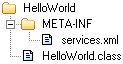
\includegraphics[width=0.3\textwidth]{HelloWorldStruktur.jpg}
\caption{\Webservice{HelloWorld}-Webservice: Dateistruktur}
\label{fig:HelloWorldStruktur}
\end{figure}

Die Klasse \Code{HelloWorld} besitzt nur die Methode \Code{SayHello}, die den \Datentyp{String} \Code{Hello World!} zur�ckgibt. Sie wird in Listing \ref{lst:HelloWorldJava} gezeigt. 

\lstset{language=Java, basicstyle=\footnotesize, showstringspaces=false, tabsize=2}
\lstinputlisting[label=lst:HelloWorldJava,caption=\Webservice{HelloWorld}-Webservice: Java-Klasse \Code{HelloWorld}]{DVD/Listings/HelloWorld/HelloWorld.java}

%\chapter{Netzwerkverkehr beim Aufruf von \Webservice{PersonFactory}}
\label{cha:SOAPNachrichten}

\section{SOAP-Request}
Listing \ref{lst:SOAPRequest} zeigt die mitgeschnittene SOAP-Anfrage per HTTP an den Webservice \Webservice{PersonFactory}. Wie am Ende von Kapitel \ref{cha:Einleitung} beschrieben, wird die eigentliche SOAP-Nachricht mittels des HTTP-\Eingabe{POST}-Befehls (Zeile 1) an den Webservice unter der angegebenen URL (Zeile 1) auf dem Server (Zeile 5) geschickt. In Zeile 3 wird �ber den Befehl \Eingabe{SOAPAction} �bermittelt, welche Funktion des Webservice (in diesem Fall \Code{CreatePerson}) aufgerufen werden soll. Die XML-Nutzlast (Zeilen 8--18) besteht dann aus einer einfachen SOAP-Nachricht aus \XMLElement{Envelope}, \XMLElement{Header} und \XMLElement{Body}, die einen RPC durchf�hrt. Die aufzurufenden Funktion wird noch einmal im SOAP-\XMLElement{Body} in Zeile 15 definiert.


\lstset{language=XML, basicstyle=\footnotesize, showstringspaces=false, tabsize=2}
\lstinputlisting[label=lst:SOAPRequest,caption=SOAP-Request an \Webservice{PersonFactory} per HTTP]{DVD/Listings/PersonFactorySOAPRequest.txt}

\section{SOAP-Response}
Die Antwort des \Webservice{PersonFactory}-Webservice zeigt Listing \ref{lst:SOAPResponse}. Sie beginnt in Zeile 1 mit dem HTTP-Statuscode 200, der die Anfrage als erfolgreich kennzeichnet. Die eigentliche Nutzlast in Form von XML-Daten (Zeile 3) folgt dann ab Zeile 7. Sie besteht aus dem Element \XMLElement{Person} und seinen Unterelementen, umschlossen vom Element \XMLElement{CreatePersonRepsonse}, das die Antwort-Nachricht aus der WSDL repr�sentiert.

\lstset{language=XML, basicstyle=\footnotesize, showstringspaces=false, tabsize=2}
\lstinputlisting[label=lst:SOAPResponse,caption=SOAP-Response von \Webservice{PersonFactory} per HTTP]{DVD/Listings/PersonFactorySOAPResponse.txt}

%\chapter{Fazit und kritische Bewertung}
\label{cha:Fazit}
Lorem ipsum dolor sit amet, consectetuer adipiscing elit. Nulla ac ipsum a metus viverra tempor. Nunc sem. Nulla nec urna eu nibh vehicula convallis. Integer ac turpis. Donec mauris enim, dignissim quis, scelerisque ac, rhoncus id, sapien. Donec turpis felis, cursus in, varius vitae, mollis ac, lorem. Integer a dui sit amet eros nonummy aliquet. Donec egestas adipiscing tellus. Nulla iaculis. Aliquam erat volutpat. Curabitur posuere, eros vitae accumsan semper, risus erat viverra erat, eu vehicula mi leo at elit. Fusce luctus. Fusce vehicula pretium diam. Nunc sed arcu ut erat suscipit fermentum.

Proin id magna eu sem tincidunt feugiat. Sed tincidunt massa sed eros. Fusce condimentum eros et lectus. Pellentesque lectus tortor, mattis in, dapibus a, lobortis ut, justo. Sed id dolor ut nibh varius ultrices. Quisque tincidunt nisl vel nibh. Suspendisse sodales massa non magna. In porttitor augue nonummy nunc. Nam quis enim quis ante dapibus interdum. Morbi nec neque. Fusce pharetra consectetuer magna. Etiam laoreet, augue nec lacinia ornare, risus purus lobortis erat, eu consequat urna orci vel arcu. Integer cursus, augue sed tempor dapibus, erat tortor rutrum elit, sit amet fermentum purus neque vitae tortor. Donec vulputate, ipsum vel viverra pretium, purus orci mattis nulla, nec tincidunt leo metus sed ipsum. Fusce eget lectus sed lectus molestie tincidunt. Etiam tincidunt urna eget tortor.

Sed sit amet magna at lectus interdum blandit. Proin vitae metus eget leo bibendum ornare. Morbi sit amet nisl ac odio accumsan laoreet. Etiam luctus massa vel enim. Vestibulum nulla tellus, viverra at, malesuada vel, volutpat quis, lorem. Vestibulum quis nulla. Curabitur neque nibh, bibendum vel, eleifend sit amet, euismod at, leo. Duis auctor lobortis justo. Donec in tortor vel nibh rutrum pellentesque. Curabitur blandit pede quis neque. Nam sem eros, ornare a, pretium eget, condimentum sed, leo. Curabitur orci felis, elementum eget, aliquet vel, porta id, velit. Etiam justo neque, rhoncus quis, elementum vel, auctor vitae, urna.




% Literaturverzeichnis -----------------------------------------------------
%		Das Literaturverzeichnis wird aus der Datenbank Bibliographie.bib 
% 	erstellt. Die genaue Verwendung von bibtex wird hier jedoch nicht erkl�rt.
%		Link: http://de.wikipedia.org/wiki/BibTeX
% --------------------------------------------------------------------------
\bibliography{Bibliographie}							% Aufruf: bibtex FHWTVorlage
\bibliographystyle{natdin}									% DIN-Stil des Literaturverzeichnisses

%\chapter*{Erkl�rung des Autors}
%\addcontentsline{toc}{chapter}{Erkl�rung des Autors}
\addchap{Eidesstattliche Erkl�rung}
Ich versichere hiermit, dass ich meine Diplomarbeit mit dem Thema
\begin{quote}
\textit{\titel} \textit{\untertitel}
\end{quote}
selbst�ndig verfasst und keine anderen als die angegebenen Quellen und Hilfsmittel benutzt habe. Die Arbeit wurde bisher keiner anderen Pr�fungsbeh�rde vorgelegt und auch nicht ver�ffentlicht.

Die Ergebnisse der Arbeit stehen ausschlie�lich dem auf dem Deckblatt angef�hrten Unternehmen zur Verf�gung (\textbf{Arbeit mit Sperrvermerk}).

Mir ist bekannt, dass ich meine Diplomarbeit zusammen mit dieser Erkl�rung fristgem�� nach Vergabe des Themas in dreifacher Ausfertigung und gebunden im Pr�fungsamt der FHWT abzugeben oder sp�testens mit dem Poststempel des Tages, an dem die Frist abl�uft, zu senden habe.\\[6ex]

Vechta, den \today


\rule[-0.2cm]{5cm}{0.5pt}

\textsc{\autor} 
	% Selbst�ndigkeitserkl�rung 

% Anhang -------------------------------------------------------------------
%		Die Inhalte des Anhangs werden analog zu den Kapiteln inkludiert.
%		Dies geschieht in der Datei Anhang.tex
% --------------------------------------------------------------------------
\begin{appendix}
	\clearpage
	\pagenumbering{roman}
	\chapter{Anhang}
\label{sec:Anhang}

% Rand der Aufz�hlungen in Tabellen anpassen
\setdefaultleftmargin{1em}{}{}{}{}{}

%\appendixtoc
\section{Liste m�glicher Aktivit�ten der BPEL}
\label{sec:ListeBPELAktivitaeten}

Die folgenden Listen basieren auf \citep[Abschnitt~10~u.~11]{OASIS2007a}.

\small

\small
\begin{longtable}{|p{0.14\textwidth}|p{0.43\textwidth}|p{0.35\textwidth}|}
\caption{Ausgew�hlte elementare BPEL-Aktivit�ten} \\
\hline
\label{tab:ListeBPELAktivitaetenElementar}
\textbf{Aktivit�t} & \textbf{Beschreibung} & \textbf{Beispiel} \\
\hline
\XMLElement{invoke} & 
Aufruf einer Operation eines Webservice. Dabei wird zwischen \Fachbegriff{One-way}- und \Fachbegriff{Request-response}-Kommunikation unterschieden. Eventuelle Input- und Output-Nachrichten werden hierbei angegeben. \XMLElement{invoke}-Elemente k�nnen weitere Elemente (wie \zB \XMLElement{faultHandler} zur Fehlerbehandlung) beinhalten. & 
\vspace{-0.8cm}
\begin{verbatim}
<invoke 
  partnerLink="PLName"
  portType="PTName"
  operation="OName"
  inputVariable="VarName"
  outputVariable="VarName">
\end{verbatim}\\
\hline
\XMLElement{receive} & Empf�ngt eine Nachricht von einem Partner. Dazu muss die Operation angegeben werden, die der Prozess anbietet um die Nachricht entgegenzunehmen. Die Nachricht kann in einer \XMLElement{variable} gespeichert werden. & 
\vspace{-0.8cm}
\begin{verbatim}
<receive 
  partnerLink="PLName"
  portType="PTName"
  operation="OName"
  variable="VarName">
\end{verbatim}\\
\hline
\XMLElement{reply} & Antwortet auf die Nachricht eines Partners (nur sinnvoll bei \Fachbegriff{Request-Response}-Kommunikation). & 
\vspace{-0.8cm}
\begin{verbatim}
<reply 
  partnerLink="PLName"
  portType="PTName"
  operation="OName"
  variable="VarName">
\end{verbatim}\\
\hline
\XMLElement{assign} & Zuweisung von Werten zu Variablen. &
\vspace{-0.8cm}
\begin{verbatim}
<assign>
  <copy>
    <from>
      <literal>
        <![CDATA[Wert]]>
      </literal>
    </from>
    <to variable="myVar" />
 </copy>
</assign>
\end{verbatim} \\
\hline
\XMLElement{throw} & Signalisierung eines Fehlers (analog zu Programmiersprachen). & 
\vspace{-0.8cm}
\begin{verbatim}
<throw 
  faultName="FName" 
  faultVariable="VarName">
\end{verbatim} \\
\hline
\XMLElement{wait} & L�sst den Prozess eine gewisse Zeit lang warten. & 
\vspace{-0.8cm}
\begin{verbatim}
<wait>
  <until>
    '2002-12-24T18:00'
  </until>
</wait>
\end{verbatim} \\
\hline
\XMLElement{exit} & Beendet den Prozess sofort. & 
\vspace{-0.8cm}
\begin{verbatim}
<exit>
\end{verbatim} \\
\hline
\end{longtable}

\small
\begin{longtable}{|p{0.14\textwidth}|p{0.43\textwidth}|p{0.35\textwidth}|}
\caption{Ausgew�hlte strukturierte BPEL-Aktivit�ten} \\
\hline
\label{tab:ListeBPELAktivitaetenStrukturiert}
\textbf{Aktivit�t} & \textbf{Beschreibung} & \textbf{Beispiel} \\
\hline
\XMLElement{sequence} & Sequentielles Abarbeiten der angegebenen Aktivit�ten. & 
\vspace{-0.8cm}
\begin{verbatim}
<sequence>
  <invoke>...</invoke>
  <invoke>...</invoke>
</sequence>
\end{verbatim}\\
\hline
\XMLElement{flow} & Paralleles Abarbeiten der angegebenen Aktivit�ten. & 
\vspace{-0.8cm}
\begin{verbatim}
<flow>
  <invoke>...</invoke>
  <invoke>...</invoke>
</flow>
\end{verbatim}\\
\hline
\XMLElement{if} & Konditionale Abfragen (vergleichbar zur Programmierung). & 
\vspace{-0.8cm}
\begin{verbatim}
<if>
  <condition>
    ...
  </condition>
  <sequence>
    ...
  </sequence>
  <elseif>
    ...
  </elseif>
  <else>
    ...
  </else>
</if>
\end{verbatim}\\
\hline
\XMLElement{while} & Wiederholung der angegebenen Aktivit�ten (vergleichbar zur Programmierung). & 
\vspace{-0.8cm}
\begin{verbatim}
<while>
  <condition>
    $orderDetails > 100
  </condition>
  <scope>...</scope>
</while>
\end{verbatim}\\
\hline
\XMLElement{scope} & Ver�ndern des Kontextes in dem die angegebenen Aktivit�ten ablaufen. So k�nnen \zB neue Variablen deklariert oder eine andere Fehlerbehandlung definiert werden. Das \XMLElement{scope}-Element stellt eigentlich keine Aktivit�t dar, soll hier aber trotzdem erw�hnt werden. & 
\vspace{-0.8cm}
\begin{verbatim}
<scope>
  <faultHandlers>
    ...
  </faultHandlers>
  <flow>
    <invoke>...</invoke>
  </flow>
</scope>
\end{verbatim}\\
\hline
\end{longtable}

\normalsize

\begin{longtable}{|m{10cm}|m{3cm}|}
\caption{Elemente der Ereignisgesteuerten Prozesskette} \\
\hline
\label{tab:ElementeDerEreignisgesteuertenProzesskette}
\textbf{Element} & \textbf{Symbol}\\
\hline
\textbf{Funktion} 

Funktionen beschreiben T�tigkeiten, die im Verlauf des Gesch�ftsprozesses anfallen. Sie k�nnen von Mitarbeitern oder einem Informationssystem durchgef�hrt werden und ben�tigen evtl. Ressourcen, die ihnen zugewiesen werden. 

Beispiele: \textit{Auftrag anlegen}, \textit{Rechnung schreiben}, \textit{Konto abschlie�en} & 
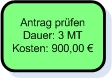
\includegraphics[width=3cm]{EPK-Funktion.jpg} \\
\hline
\textbf{Ereignis} 

Ereignisse sind betriebswirtschaftlich relevante Ereignisse, die den Gesch�ftsprozess in irgendeiner Weise steuern oder beeinflussen. Ereignisse sind immer Ausl�ser oder Ergebnisse von Funktionen. Ein Gesch�ftsprozess beginnt und endet stets mit einem Ereignis. 

Beispiele: \textit{Auftrag eingetroffen}, \textit{�berweisung get�tigt}, \textit{Rechnung erstellt} & 
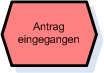
\includegraphics[width=3cm]{EPK-Ereignis.jpg} \\
\hline
\textbf{Operatoren} 

Operatoren steuern den Kontrollfluss eines Gesch�ftsprozesses. Sie machen \zB deutlich, dass eine Funktion mehrere Ereignisse ausl�st, oder zeigen alternative Vorgehensweisen an. Es gibt drei Operatoren (v.\,l.\,n.\,r.\,): UND, ODER und XODER (exklusives ODER). & 
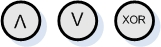
\includegraphics[width=3cm]{EPK-Operatoren.jpg} \\
\hline
\textbf{Organisationseinheit} 

Organisationseinheiten werden Funktionen zugeordnet und beschreiben, wo die Funktionen ausgef�hrt werden bzw. wer sie ausf�hrt. Die Bezeichnung der Symbole enth�lt zus�tzlich zur Abteilung noch die Namen der Mitarbeiter.

Beispiele: \textit{Vertrieb}, \textit{Personal}, \textit{Produktion} & 
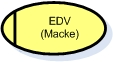
\includegraphics[width=3cm]{EPK-Organisationseinheit.jpg} \\
\hline
\textbf{Informationsobjekt} 

Auch Informationsobjekte werden Funktionen zugewiesen und beschreiben die von diesen ben�tigten oder erstellten Informationen. Dabei sind s�mtliche Formen von Informationen auf verschiedenen Datentr�gern m�glich und nicht etwa nur digitale Daten. Die Bezeichnung der Symbole enth�lt zus�tzlich das Informationssystem, aus dem die Informationen stammen.

Beispiele: \textit{Kundendatenbank}, \textit{Versicherungsantrag}, \textit{Rechnung} & 
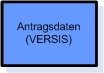
\includegraphics[width=3cm]{EPK-Informationen.jpg} \\
\hline
\textbf{Prozesswegweiser}

Mit Prozesswegweisern werden Prozesse, die in anderen EPKs beschrieben sind, referenziert. So k�nnen \zB un�bersichtliche Prozesse in Teilprozesse gegliedert und h�ufig verwendete Prozesse an zentraler Stelle modelliert werden. Prozesswegweiser stehen in einer EPK immer anstelle von Funktionen. & 
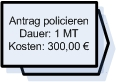
\includegraphics[width=3cm]{EPK-Prozesspfad.jpg} \\
\hline
\end{longtable}

\section{Verwendete Werkzeuge}
\label{sec:Werkzeuge}
BEREITS BEARBEITET!\\
Im Folgenden werden die Hardware und Software vorgestellt, welche die Autoren zum Erstellen dieser Arbeit und vor allem zur Entwicklung der App verwendet haben. Es wurden ausschliesslich Open-Source-Programme eingesetzt.\\
Hier benutzte Beschreibungen k�nne von Website (offizielle Site der Software, Wikipedia...) �bernommen sein. Dieser Abschnitt dient zur Information f�r die verwendeten Werkzeuge.
\subsection{Software}
\begin{itemize}
\item \textbf{Eclipse} \\
Eclipse (von englisch eclipse Sonnenfinsternis, Finsternis, Verdunkelung) ist ein quelloffenes Programmierwerkzeug zur Entwicklung von Software verschiedenster Art. Urspr�nglich wurde Eclipse als integrierte Entwicklungsumgebung f�r die Programmiersprache Java genutzt, aber mittlerweile wird es wegen seiner Erweiterbarkeit auch f�r viele andere Entwicklungsaufgaben eingesetzt. F�r Eclipse gibt es eine Vielzahl sowohl quelloffener als auch kommerzieller Erweiterungen.
Eclipse selbst basiert auf Java-Technik, seit Version 3.0 auf einem sogenannten OSGi-Framework namens Equinox.\\
\\
Eclipse wurde als Grundwerkzeug f�r die App-Programmierung benutzt. In den ersten beiden Studienjahren haben wir mit Eclipse Java-Applikationen entwickelt.\\ \\

\includegraphics[height=3cm]{eclipse_logo.png} \\
Website: \url{http://www.eclipse.org/} \\

\item \textbf{\LaTeX} \\
Diese Arbeit wurde mit {\LaTeX} geschrieben. Als Distribution und Editor wurde auf dem Mac OS Mountain Lion TexShop verwendet, auf Basis von Linux ????????????. \\
Websites: \url{http://pages.uoregon.edu/koch/texshop/}
\end{itemize}

\subsection{Hardware}
ALLES HIER IST AKUTELL\\
Ausser die Sch*** Tabelle, die sich nicht formatieren lassen m�chte...\\
\begin{itemize}

\item \textbf{Galaxy Nexus} \\
Auf diesem Smartphone l�uft das brandaktuelle Andoid OS 4.1.1 (Nelly Bean).\\
\begin{tabular}[t]{|l|l|c|} \hline
 \cellcolor{darkgrey} &  \cellcolor{darkgrey} & \\
\cellcolor{darkgrey} \multirow{-2}{3cm}{\textbf{Bezeichnung}} &
\cellcolor{darkgrey} \multirow{-2}{6cm}{\textbf{Version}} &  \\
model number & Galaxy Nexus & \\ \cline{1-2}
Android-Version & 4.1.1 (Jelly Bean) &\\ \cline{1-2}
Baseband-Version & I9250XXLF1 &\\   \cline{1-2}
Kernel-Version & 3.0.31-g6fb96c9 &\\  \cline{1-2}
Build number & JR003C.I9250XWLH2 & \\  \cline{1-2}
Screen Resolution & 1280 x 720 pixel & \\ \cline{1-2}
diagonal & 4.65 inch & \multirow{-8}{6cm}{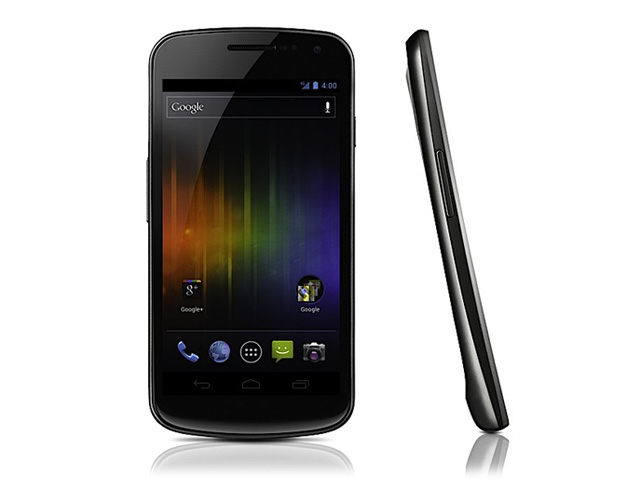
\includegraphics[width=6cm]{galaxynexus.png} }\\  \hline 
\end{tabular}\\



\item \textbf{Gr�enis Phone...} \\
\begin{tabular}[t]{|l|l|} \hline
 \rowcolor{darkgrey} &\\
\rowcolor{darkgrey}
\multirow{-2}{3cm}{\textbf{Bezeichnung}} &
\multirow{-2}{10cm}{\textbf{Version}} \\
model number & \\ \hline 
Android-Version & \\  \hline 
Baseband-Version &  \\  \hline 
Kernel-Version & \\  \hline 
Build number &  \\  \hline 
Screen Resolution &\\  \hline 
diagonal & \\  \hline 
\end{tabular}\\


\end{itemize}

\end{appendix}


% Index --------------------------------------------------------------------
%		Zum Erstellen eines Index, die folgende Zeile auskommentieren.
% --------------------------------------------------------------------------
%\printindex		% Index hier einf�gen

\end{document}
